\subsection{Overview of phylodynamics}

\subsubsection{Phylogenetic trees}

In evolutionary biology, a \defn{phylogeny}, or \defn{phylogenetic tree}, is a
graphical representation of the the evolutionary relationships among a group of
organisms or species (generally, \defn{taxa}). Phylogenies consist of nodes,
representing taxa, and edges or branches, which connect taxa to their
evolutionary ancestors and descendants. The \defn{tips} of a phylogeny, that
is, the nodes without any descendants, correspond to \defn{extant}, or
observed, taxa, while the \defn{internal nodes} correspond to their extinct
common ancestors. Phylogenies may have a \defn{root}, which is a node with no
descendants distinguished as the most recent common ancestor of all the extant
taxa. When such a root exists, the tree is referred to as being \defn{rooted};
otherwise, it is \defn{unrooted}. The structural arrangement of nodes and edges
in the tree is referred to as its \defn{topology}. The branches of the tree may
have associated lengths, representing either calendar time or genetic distance
between ancestors and their descendants. 

A phylogeny with branch lengths in calendar time units is often referred to as
\defn{time-scaled}. In a time-scaled phylogeny, the internal nodes can be
mapped onto a timeline by using the tips of the tree, which usually map to the
present day, as a reference point~\autocite{nee1992tempo}. The corresponding
points on the timeline are called \defn{branching times}. These concepts are
illustrated in Figure~\ref{fig:speciestree}.

\begin{figure}[ht]
  \centering
  \label{fig:speciestree}
  \includegraphics{speciestree}
  \caption[Illustration of a rooted, time-scaled phylogeny]{Illustration of a
    rooted, time-scaled phylogeny. The tips of the tree, which represent extant
    taxa, are placed at the present day on the
    time axis. Internal nodes, representing extinct common ancestors to the
    extant taxa, fall in the past. The topology of the tree indicates that cats
    and dogs are the most closely related pair of species, whereas fish is most
    distantly related to any other node in the tree.}
\end{figure}

\subsubsection{Species trees and transmission trees}

A \defn{species tree} is a particular type of phylogeny in which the taxa are
species, and the branching times correspond to historical speciation events. In
general, we do not have access to the true tree relating a particular group of
extant species, as this would imply certain knowledge of speciation events in
the distant past. Therefore, all species trees considered by researchers are
estimates, based on the genetic or phenotypic similarity of the extant taxa,
the fossil record, or both. We discuss some of the challenges associated with
this estimation in subsection \ref{subsec:treeconv} below. However, for the
moment, we ignore these complications and suppose that we know the true species
tree.

The process of speciation, which causes branching in a species tree, often
occurs by an \defn{allopatric} process, where a sub-population of organisms is
isolated from the original population by a geographic
barrier~\autocite{coyne2004speciation}. Over time, the two populations diverge
genetically, eventually resulting in two distinct species.

\subsubsection{Gene trees and viral phylogenies}

\subsubsection{Using gene trees to estimate species trees}

\subsubsection{Tree shapes}

\subsection{Contact networks}

\subsubsection{Overview and epidemiology}

Epidemics spread through populations of hosts through \defn{contacts} between
those hosts. The definition of contact depends on the mode of transmission of
the pathogen in question. For an airborne pathogen like influenza, a contact
may be simple physical proximity, while for a sexually transmitted pathogen
like HIV, contacts would be sexual partnerships. A \defn{contact network} is a
graphical representation of a host population and the contacts among its
members. The \defn{nodes} in the network represent hosts, and \defn{edges}
represent contacts between them. 

Edges in a contact networks may be \defn{directed}, representing one-way
transmission risk, or \defn{undirected}, representing symmetric transmission
risk. For example, a network for an airborne epidemic would use undirected
edges, because the same physical proximity is required for a host to infect or
to become infected. However, a blood-borne infection spread through
transfusions would use undirected edges, since the donor has no chance of
transmitting to the recipient. Directed edges are also useful when the
transmission risk is not equal between the hosts, such as with HIV
transmission, where acting as the receptive partner carries a higher risk of
infection than acting as the insertive partner. In this case, a contact could
be represented by two directed edges, one in each direction between the two
hosts, with the edges annotated by what kind of risk they imply. In fact, it is
possible to represent an undirected edge by two symmetric directed edges. For
this reason, we consider only contact networks with directed edges in the
sequel. A directed contact network is shown in Figure \ref{fig:contactnet}
(left).

The path an epidemic takes through a contact network determines the topology of
the transmission tree relating the infected hosts. The initially infected node
who introduces the epidemic becomes the root of the tree. Each time a
transmission occurs, the lineage corresponding to the donor host in the tree
splits into two, representing the recipient lineage and the continuation of the
donor lineage. This correspondence is illustrated in figure
\ref{fig:contactnet}. It's important to note that, although the order and
timing of transmissions determines the tree topology uniquely, the converse
does not hold. That is, there are generally several orders of infection which
could lead to the same topology, since the labels on the internal nodes of the
tree are not available to the researcher.

\begin{figure}[ht]
  \centering
  \label{fig:contactnet}
  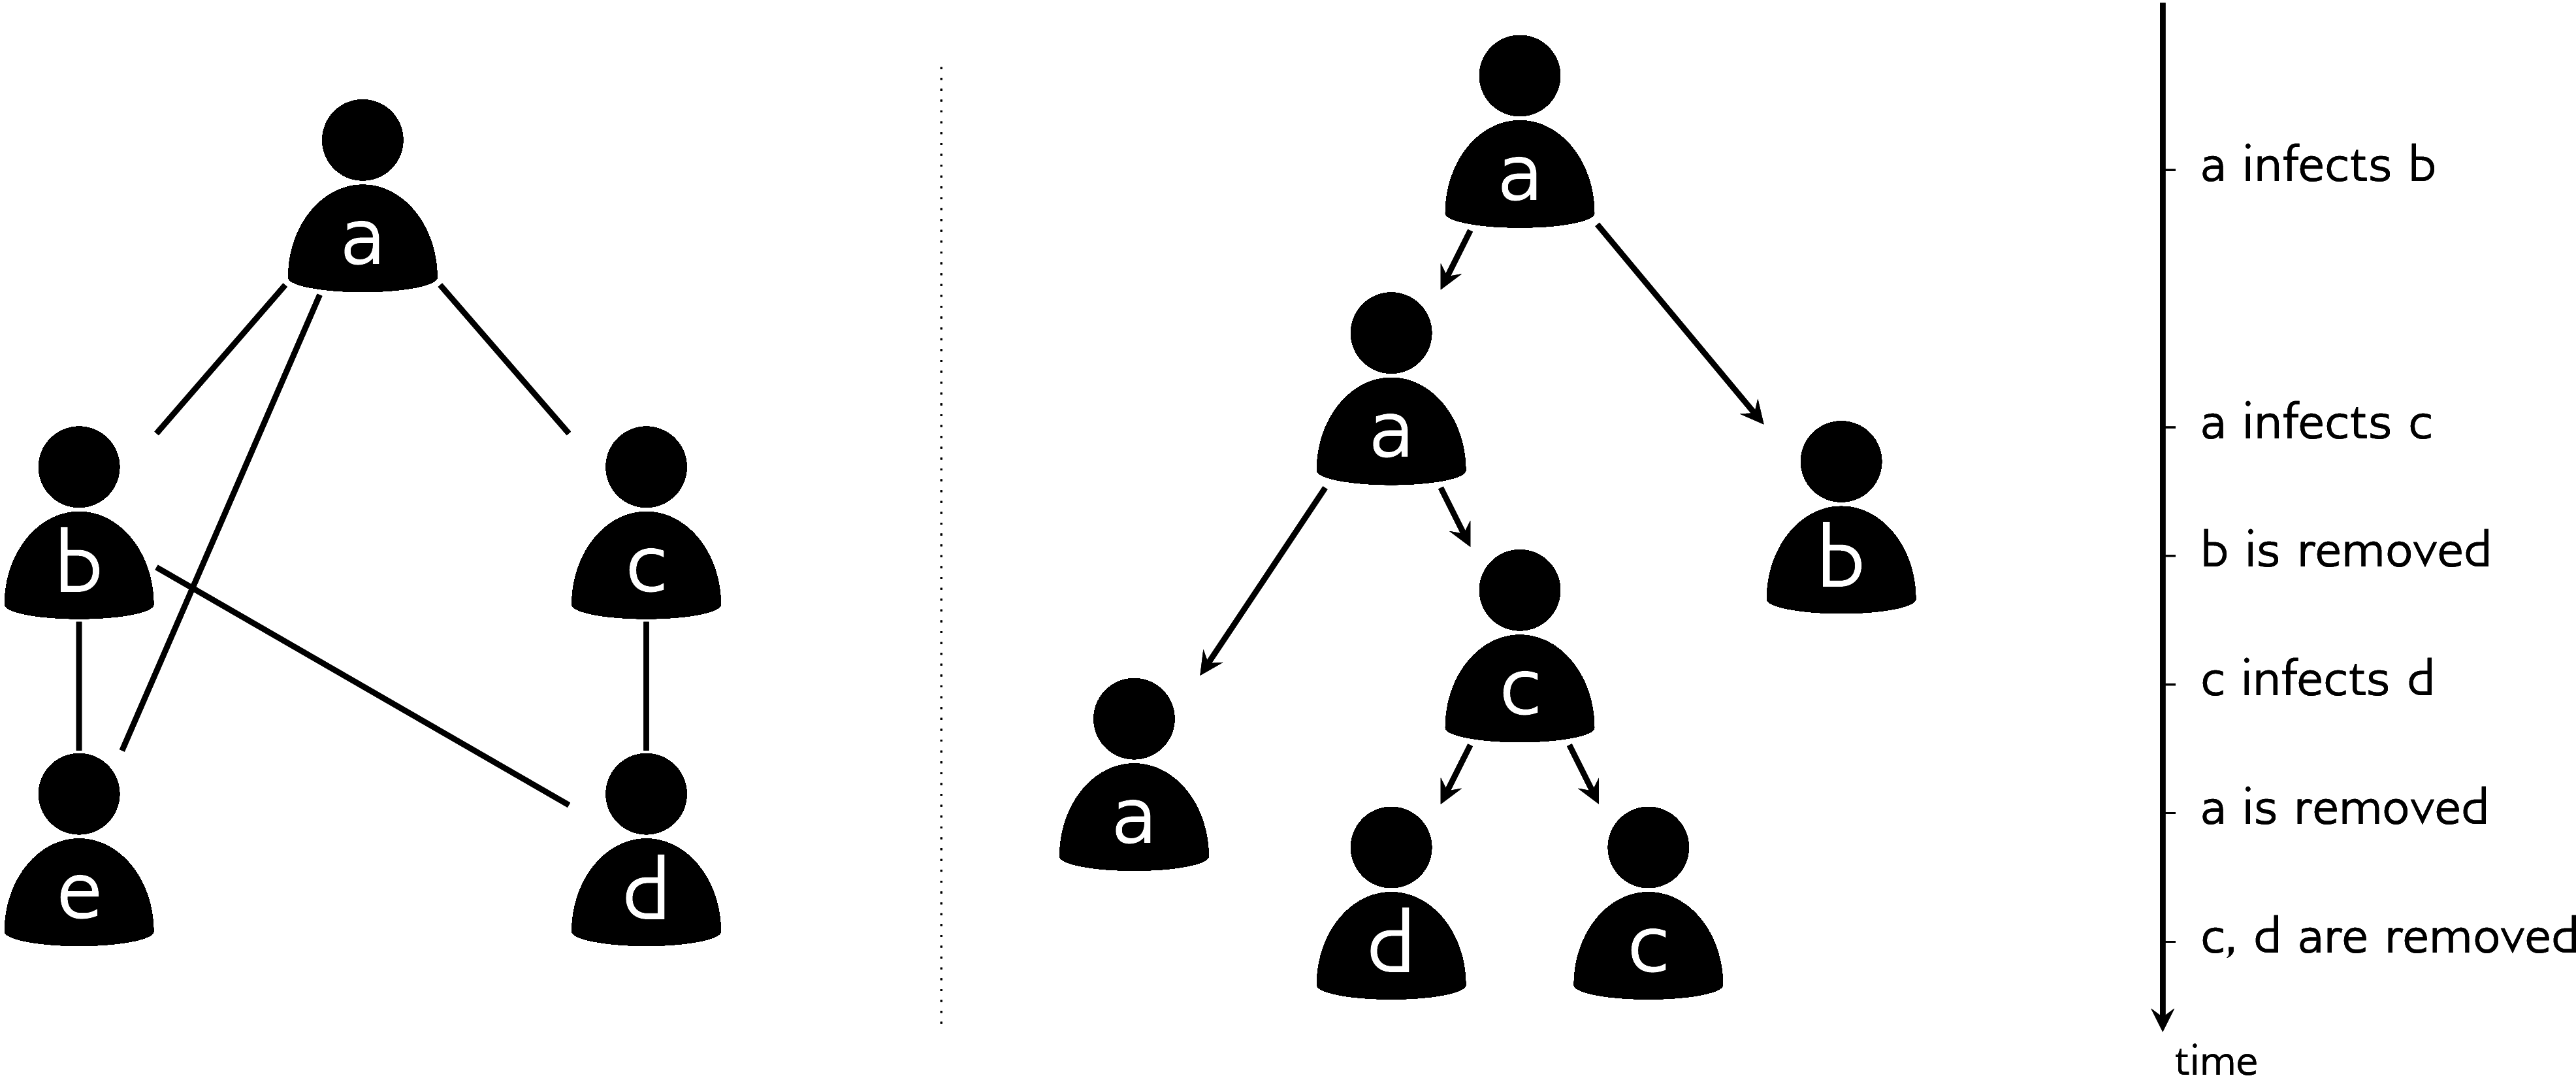
\includegraphics{contactnet}
  \caption[Illustration of a epidemic spread over a contact network]
  {Illustration of epidemic spread over a contact network. On the left, a
   contact network with five hosts, labelled A through E. Directed edges
   indicate six symmetric contacts among the hosts. Coloured, bolded edges
   represent transmissions. The epidemic began at node A, who transmitted to
   nodes B and C. Node C further transmitted to node D, and node E was not
   infected. On the right, the transmission tree topology corresponding to this
   scenario.}
\end{figure}

\subsubsection{Generative models}

%Now, consider a phylogeny not of macro-organisms, but of RNA viruses. Many of
%these, such as the human immuno-deficiency virus (HIV), evolve rapidy enough
%that populations can accumulate measurable genetic changes on time scales of
%months or years~\autocite{drummond2003measurably}. Because viruses cannot exist
%for long outside their hosts, the host replaces the outside world as the
%``environment'' in which evolution takes place. 
%
%In this light, striking parallels can be drawn between immunological and
%epidemiological processes at the host level, and the evolutionary processes
%studied in population genetics~\autocite{grenfell2004unifying}. For example,
%both the host immune response~\autocite{mcmichael2001cellular} and the presence
%of anti-retroviral drugs~\autocite{??} exert directional selection on the viral
%population within a single host. Transmission, where a sub-population of
%virions from the donor host is ``geographically'' isolated in the recpient,
%closely mirrors the allopatric speciation process and causes a branching point
%in the viral phylogeny (although this may not correspond exactly to the time of
%transmission, as discussed in the next section). Consequently, any factor which
%influences transmission dynamics, such as the virus' mode of transmission or
%the population structure of its hosts, in turn affects the shape of the
%phylogeny. The study of this interaction between host-level factors and viral
%phylogies is known as \defn{phylodynamics}~\autocite{grenfell2004unifying}. 
%
%In particular, if a time-scaled phylogeny is constructed where all viruses from
%the same host are collapsed into a single taxon, we might expect the branching
%time relating the two hosts to correspond to the time of transmission. Of
%course, this will only be the case if the two hosts' infections indeed diverged
%allopatrically at the time of transmission, and not sympatrically within the
%donor host at some previous time. This limitation, and others, in interpreting
%the branching times of the viral phylogeny as transmission times, are discussed
%in the next section. Nevertheless, even taking these limitations into account,
%the relationship between branching times in the phylogeny and transmission
%times in the population theoretically implies that the evolutionary history of
%the virus is informative about the biology and epidemiology of its hosts. In
%other words, information about, for example, transmission patterns, might be
%inferred from the viral phylogeny. Phylodynamic methods are intended to
%complement more traditional approaches to gathering epidemiological data, such
%as population surveys.
%
%
%\subsection{Sources of error in phylodynamics}
%\label{subsec:treeconv}
%
%In general, the exact topology and branch lengths of a phylogeny relating
%arbitrary taxa are not known and must be estimated. Such estimation is most
%often carried out using some type of genetic data sampled from each of the
%taxa, either amino acid sequences or gene orders. The resulting phylogeny, also
%known as a \defn{gene tree}, differs from the time-scaled \defn{species tree}
%which would contain complete information about past speciation events. In
%viral phylogenetics, the gene tree is the viral phylogeny, constructed using
%the genetic sequences of the sampled viruses. On the other hand, the species
%tree is the \defn{transmission tree}, wherein branching times correspond
%exactly to transmission times. In general, phylodynamic methods perform
%inference based on the transmission tree, which must be inferred from a viral
%phylogeny based on the available sequence data. The inference of the viral
%phylogeny itself is not an error-free process, as accurate phylogenetic
%inference is still an active area of research. Moreover, the conversion of the
%phylogeny into a transmission tree is a process which has the potential to
%introduce at least three types of error, described below. We use the terms
%``gene tree'', ``viral phylogeny'', and ``phylogeny'' interchangably, as well
%as the terms ``species tree'' and ``transmission tree''.
%
%Firstly, the branch lengths of the gene tree are measured in genetic distance,
%and must be somehow converted to units of calendar time used in the species
%tree. If we assume a constant rate of evolution along the whole tree (a
%\defn{strict molecular clock}), then this conversion is straightforward - we
%simply divide each of the branch lengths by the rate of evolution. However, it
%is well known that rates of evolution are neither constant over time nor
%constant between lineages, and the general problem of time-scaling a
%phylogenetic tree is still an active area of research. Phylodynamic inference
%relies on the assumption of a correctly time-scaled tree, and violations of
%this assumption can mislead parameter estimates.
%
%A second limitation which has perhaps greater potential to mislead phylodynamic
%inference is the potential discordance between the gene tree and the species
%tree. In an allopatric speciation, some of the genetic diversity separating the
%two eventual species may already have been present in the population
%\emph{before} the geographic isolation occured. In that case, the branching
%time in the gene tree, which indicates the time when two genetically distinct
%versions of the gene, may be earlier than the branching point in the species
%tree. In evolutionary biology, this phenomenon is referred to as
%\defn{incomplete lineage sorting}. Furthermore, if there was substantial
%variation within a population which underwent two or more speciation events in
%close succession, the order in which the species diverged may be different from
%the order in which their distinct genes arose in the original heterogeneous
%population. In this case, the topology of the species tree would be different
%from that of the gene tree. 
%
%Finally, there is the problem of rooting the tree, that is, identifying the
%node corresponding to the most recent common ancestor of all the sampled
%viruses. The choice of root influences the temporal order of the internal
%nodes in the phylogeny. If the tips are constrained to the present day, or some
%other fixed sampling time, the branch lengths in the species tree must also be
%altered to accomodate the choice of root. 
%
%To our knowledge, there has been no theoretical exploration of the quantitative
%effect of any of these sources of error on the accuracy of phylodynamic
%inference. Most phylodynamic studies assume, implicitly or explicitly, that the
%viral phylogeny provides the same information as the transmission tree, and
%errors introduced by this assumption are generally ignored. Studies employing
%Bayesian methods eliminate some of the uncertainty associated with constructing
%the viral phylogeny, but this does not account for the error introduced in the
%phylogeny-to-transmission-tree conversion process. Our work does not take a
%Bayesian approach to inferring the phylogeny, and therefore is susceptible to
%all the sources of error discussed here.
%
%\subsection{Contact networks}
%
%Compartmental models of epidemic growth and spread often assume that human
%populations are homogeneously mixed, that is, any person in the population is
%equally likely to transmit the infection to any other. More sophisticated
%models allow for the population to be divided into groups with higher or lower
%contact rates, but these still do not account for individual variation or
%population structure within compartments. In reality, and especially for
%sexually-transmitted infections such as HIV, this assumption of homogeneity is
%not realistic. There is substantial variation in the number of contacts per
%individual, and potential transmissions are limited by geographic proximity.
%The aim of using contact networks is to remove these unrealistic assumptions by 
%explicitly simulating each individual in a population, along with the contacts
%they have which could possibly lead to a transmission.
%
%A \defn{contact network} is a graphical representation of a population over
%which an epidemic can spread. Contact networks consist of nodes and edges,
%where the nodes represent people, and edges represent contacts. An edge between
%two nodes indicate that transmission is possible between the two corresponding
%individuals. For example, if we are considering an HIV transmission network,
%the edges may represent sexual contacts or individuals sharing injection drug
%paraphernalia. For an airborne pathogen such as influenza, an edge may simply
%indicate that the two people were in the same room. The edges in a contact
%network may be undirected, indicating that all contacts could possibly transmit
%to each other, or directed, indicating that transmission risk is one-way. It is
%possible to simulate an undirected network using directed edges by simply
%including two directed edges, one in either direction, for each single directed
%edge. Therefore, we exclusively consider directed contact networks here.
%
%Contact networks have been studied extensively in a variety of social,
%economic, and public health contexts. However, investigation of the effects of
%contact network structures on viral phylogenies have been much more limited.
%Existing studies have to focused on a few broad classes of contact network, and
%how phylogenies deriving from these networks have
%differed~\autocite{leventhal2012inferring, colijn2014phylogenetic,
%robinson2013dynamics}. To demonstrate our method, we focus on the same three
%contact network types as studied in~\autocite{leventhal2012inferring}, namely
%Erdos-Renyi (ER) graphs, Barabasi-Albert (BA) graphs, and Watts-Strogatz (WS)
%graphs. ER graphs, also known as random graphs, are the simplest generative
%graph model~\autocite{erdos1960evolution}. They have a single parameter, $p$,
%which gives the probability of any edge occuring in the network. BA
%graphs~\autocite{barabasi1999emergence} model a preferential attachment process
%where nodes with high degree tend to attract more connections. They have two
%parameters, $m$ and $\alpha$, and are constructed by repeatedly adding new
%nodes with $m$ outgoing edges to the network. An existing node $v$ in the
%network is chosen to be the endpoint of these new edges with probability
%proportional to $d(v)^\alpha$, where $d(v)$ is the degree of $v$. WS
%graphs~\autocite{watts1998collective}, also known as small-world graphs, have
%two parameters, $k$ and $p$. They are constructed by creating a ring lattice
%with $k$ edges per node, and then randomly rewiring each edge with probability
%$p$.
%
%\subsection{Approximate Bayesian computation}

%Consider a model $M$, with parameters $\theta$, which we wish to fit to some
%observed data $D$. By ``fit'', we often mean that we want to find particular
%values $\hat{\theta}$ for the parameters which optimize the likelihood of our
%data given those parameters and the model,
%\[
%  \hat{\theta} = \argmax_\theta \Pr(D | M, \theta).
%\]
%This $\hat{\theta}$ is the \defn{maximum likelihood} parameter estimate. Note
%that we are employing a common abuse of notation here, where $\Pr(\cdots)$ is
%being unsed to refer to a probabilty \emph{density} rather than a true
%probability. Alternative to maximum likelihood, we may be interested less in a
%point estimate and more in the posterior distribution of possible values of
%$\theta$ given our data, $\Pr(\theta \mid M, D)$. This will be expanded upon
%below, but for the moment, for illustrative purposes, we restrict our attention
%to the maximum likelihood problem.
%
%If the model we are fitting is sufficiently simple, it may be possible to
%calculate $\hat{\theta}$ directly, using calculus. Most models do not admit
%analytic maximum likeilhood solutions, but if the likelihood any set of
%parameters can be calculated up to a normalizing constant, then
%${\Pr(D \mid M,\theta)}$ can be optimized numerically. A wide range of
%optimization strategies exist, the choice of which to use depending on the
%complexity of the model and whether or not we have access to the gradients of
%the likelihood function with respect to each of the parameters. The majority of
%modelling problems fit into this category, and numerical optimization is
%well-developed and extremely widely used.
%
%However, there are some cases, often when the observed data is of a complex
%type, that explicitly calculating the likelihood of some observed data is
%impossible, even up to a normalizing constant. For example, suppose that we
%want to model a chess player's behaviour. We will set up a simple one-parameter
%model which describes the chess playing process.  The parameter, $a \in [0, 1]$
%indicates the player's eagerness to remove his opponent's pieces from the
%board. We can write down an algorithm for the player's behaviour under such a
%model.
%
%% TODO: don't break this over the page
%
%\begin{algorithmic}
%  \While{the game is not over}
%    \If{I can capture an opponent's piece and $\Uniform(0, 1) < a$}
%      \State{capture the piece}
%    \Else
%      \State{make any other move at random}
%    \EndIf
%  \EndWhile
%\end{algorithmic}
%
%Suppose the observed data are the ending configurations of the board, after the
%player has concluded a game against an opponent with a known value of $a$. The
%model we have designed is very simple, but it is not obvious how to calculate
%the likelihood of a particular ending configuration. Indeed, it seems that the
%only way is to enumerate every possible path the game could have taken, and
%tabulate the ending configurations of each. Clearly, this is infeasible.
%Approximate Bayesian computation was designed for situations like these, where
%exact likelihoods are not available, perhaps due to the model involving an
%algorithm or generative process.
